If a contamination incident is detected by a water utility, it will be
important to determine the time and location where the contaminant
injection occurred. Once this information is available, the current
extent of contamination within the network can be estimated and
appropriate control and clean-up strategies can be devised in order to
protect the population. The \code{inversion} subcommand included in
WST is designed to calculate a list of possible injection nodes and
times given a set of measurements that could come from manual grab
samples and/or an event detection system (EDS) like CANARY \citep{CANARY}.

Three major challenges associated with source identification
calculations are addressed by this subcommand.  
\begin{itemize}
\item First, the source
identification algorithms provided through this subcommand have to
consider measurement data that can only provide a discrete yes/no
indication of contamination at a particular sensor node and time. 
It is assumed that the current level of sensor technology can only provide
standard water quality measures such as free chlorine, conductivity,
pH, total organic carbon. Using these measurements, the EDS performs statistical
analysis to detect anomalous changes from a baseline and
provides a yes/no indication of potential contamination. Therefore,
the source identification algorithms provided through this subcommand
are designed to work with binary measurements.  
\item Second, measurement
information available from a sparse set of fixed sensors might not be
sufficient to narrow down the possible contamination nodes to a
tractable number. One strategy is to get additional measurements in
the form of manual grab samples from locations around the network to
help the source identification calculations better identify the
contamination location(s). 
The \code{grabsample} subcommand (described in Chapter \ref{chap:grabsample})
can be used to establish the best manual grab sample locations that will
provide the most useful information to help establish the likely 
source(s).
%The location of these manual grab samples
%can be carefully selected to provide maximum distinguishability
%between the possible incidents by using the \code{grabsample}
%subcommand (described in Chapter \ref{chap:grabsample}). 
The source
inversion algorithms in WST can use measurement information from both
fixed sensors and manual grab samples.
\item Third, during a contamination incident, being able to solve
the source identification problem in real-time is of utmost importance.
Therefore, all algorithms provided through this subcommand pay special 
attention to computational efficiency and typically perform source identification 
calculations within minutes on realistic large-scale networks.
\end{itemize}   
A flowchart representation of
the \code{inversion} subcommand is shown in
Figure \ref{fig:inversion_command_flowchart}. The utility network model is
defined by an EPANET 2.00.12 compatible network models (INP format) in WST.
The sensor/EDS measurements are supplied through a measurements file
(See File Formats Section \ref{formats_measFile}). Additional details
on the source inversion approach to identify the contaminant injection
location(s) is supplied by the user in the WST configuration file.

\begin{figure}[h]
  \centering
  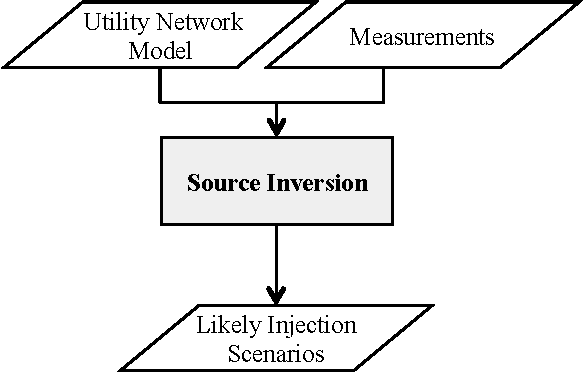
\includegraphics[scale=0.75]{graphics/inversion_flowchart.pdf}
  \caption{Contamination source identification flowchart.}
  \label{fig:inversion_command_flowchart}
\end{figure}

\section{Source Identification Formulations}\label{source_inversion_algorithms}
The \code{inversion} subcommand contains three different source identification
formulations, a Mixed Integer Programming (MIP) formulation, a
formulation based on Bayesian probability calculations and a modified
version of the Contaminant Status Algorithm by \citet{csa}. The following
subsections provide brief descriptions of these formulations. 

\subsection{MIP Formulations}
Typically, optimization based methods try to find injection candidates
that minimize the deviation between calculated values and the
measurements (e.g., least squares), penalizing any mismatch above or
below the measured values. The Mixed Integer Programming (MIP)
formulation assumes that a field sensor (or manual grab sample) would
yield a positive measurement if the contaminant concentration is above
a certain positive threshold concentration and a negative measurement
if it is below a certain negative threshold concentration. The
objective function seeks to minimize the difference between the
measured and calculated behavior according to this threshold.
%The Mixed Integer Programming (MIP) formulation assumes that a field sensor (or manual grab sample)
%would yield a positive measurement if the contaminant concentration is
%above a certain positive threshold concentration and a negative
%measurement if it is below a certain negative threshold concentration.
Therefore, if a sensor measurement (or a manual grab sample) yields a
positive measurement, any corresponding calculated concentration from
the water quality model above the positive threshold is deemed to be a
perfect fit with this measurement data. Hence, when constructing
an objective for estimation, only calculated concentrations below this
positive threshold should be minimized. Likewise, if a sensor (or
manual grab sample) yields a negative measurement, only the
corresponding calculated concentration above the negative threshold
should be minimized. Based on this idea, the base MIP formulation is presented below 
followed by descriptions of three additional variations that perform source
inversion under different assumptions. 
For more detailed information, please refer to \citet{Mann1}.


\label{sec.mip_formulation}
\begin{align}
\textrm{minimize}\qquad &\sum_{(n,t) \in \mathbf{S}_-}\mathrm{neg}_{n,t} + \sum_{(n,t) \in \mathbf{S}_+}\mathrm{pos}_{n,t} \label{eqn.milp_first_egn}\\
\textrm{subject to}\quad &Gc_{n,t} = D\mathbf{m}_R &&\forall n \in \mathbf{N}, t\in \mathbf{T} \label{eqn.milp_merlion_model}\\
&0 \le m_{n,t} \le By_n &&\forall n \in \mathbf{N},
t\in \mathbf{T} \label{eqn.milp_big_m}\\
% &m_n(t_{j-1}) \le m_n(t) &&\forall k \in \mathbf{N},
% j\in \mathbf{T}: j \neq 0 \label{eqn.mass_inj_constraint}\\
&\sum_{n \in \mathbf{N}} y_n \le I_{\max} && y_n \in \lbrace
0,1 \rbrace \label{eqn.inj_constraints}\\ &\mathrm{neg}_{n,t} \geq 0, \;\;
\mathrm{neg}_{n,t} \geq c_{n,t}-\tau _\mathrm{neg} &&\forall \left(
n,t \right) \in \mathbf{S}_- \label{eqn.milp_negative_set}\\
&\mathrm{pos}_{n,t} \geq 0, \;\; \mathrm{pos}_{n,t} \geq \tau _\mathrm{pos} -c_{n,t}
&&\forall \left(
n,t \right) \in \mathbf{S}_+. \label{eqn.milp_positive_set}
\end{align}

where $N$ is the set of all nodes, $T$ is the set of all time steps,
$S_-$ represents the set containing the node-time step pairs where the
discrete measurement is a negative detection and $S_+$ defines the set
containing the node-time step pairs where the discrete measurement is
a positive detection. The parameters $G$ and $D$ are matrices from
the Merlion water quality model. The variable $c_{n,t}$ is the
calculated concentrations from the water quality model at node $n$ and
time step $t$, $m$ is the vector of unknown time-discretized
contaminant injection profile over all node and time steps and
$m_{n,t}$ is an element in the $m_R$ vector representing unknown mass
injected at node $n$ and time step $t$. A binary variable, $y_n$,
indicates contaminant injection at node $n$ if $y_n{=}1$ and $B$ is a
reasonable upper bound on the contaminant injection mass flow rate
$m_{n,t}$. The variable $I_{\max}$ is the maximum number of possible
injection locations. The user supplies two thresholds, $\tau _\mathrm{neg}$
and $\tau _\mathrm{pos}$, which can be used as concentration set-points
indicating the presence or absence of contaminant. Having a gap
between the positive and negative threshold provides users a (buffer)
region of concentration values where really small fluctuations do not
lead to a positive measurement. Therefore, the user can specify a
higher positive threshold than the negative threshold to only flag
significant concentration changes as positive detection. The variable
$\mathrm{neg}_{n,t}$ is the non-negative difference between the modeled
concentration $c_{n,t}$ and the user supplied threshold $\tau _\mathrm{neg}$
for node-time step pairs belonging to $\mathbf{S}_-$. The variable
$\mathrm{pos}_{n,t}$ is the non-negative difference between the modeled
concentration $c_{n,t}$ and the user supplied threshold $\tau _\mathrm{pos}$
for node-time step pairs belonging to $\mathbf{S}_+$.


Equation \ref{eqn.milp_first_egn} is the MIP objective, which
minimizes the mismatch between the discrete measurements and their
corresponding concentrations calculated from the model given the
detection thresholds. Equation \ref{eqn.milp_merlion_model} is the
embedded linear water quality model (Merlion, see Section \ref{appendixMerlion} for details). 
% Note that the reduced version of this model given by equation 
% (ref) is used in place of the full model. 
Equation \ref{eqn.milp_big_m} is the big-M constraint
that enforces the bound on the maximum mass flow rate of the injections.
%\item Equation \ref{eqn.mass_inj_constraint}: Allows for the 
%case where the mass flow rate of contaminant could stay the same or increase with time.
Equation \ref{eqn.inj_constraints} is the maximum number of injections constraint, while
Equation \ref{eqn.milp_negative_set} and Equation \ref{eqn.milp_positive_set} 
are part of the reformulation of the objective function to handle the 
threshold treatment discussed above. For further details please refer to \citet{Mann1}.
They are used to 
enforce $\mathrm{neg}_{n,t}$ and $\mathrm{pos}_{n,t}$ as non-negative differences between modeled concentration and 
threshold for positive and negative measurements, $\tau _\mathrm{pos}$ and $\tau _\mathrm{neg}$, respectively. 

This base MIP formulation for
discrete measurements can be selected using the formulation option of
MIP\_discrete in the inversion block of the \code{inversion} WST
configuration file.

The source inversion problem is ill-posed with non-unique
solutions. To tackle this issue, the \code{inversion} subcommand solves
the problem multiple times, each time adding additional feasibility constraints
to exclude previously found solutions until the objective of the solution
has reduced significantly. Therefore, the final result reported by
the \code{inversion} subcommand contains a list of objective values
for each solution and the corresponding source node that was identified
for that particular solution. 

The base MIP formulation allows for any type of injection profile including the ones
shown in Figure \ref{fig:inversion_variations}. In the presence of sufficient 
measurement information, identification of any injection profile is reasonable.    
For instance, the Pulse profile in Figure \ref{fig:inversion_variations} (shown in red),
requires frequent measurements from the sensors in order to detect and characterize the injection. 
However, with relatively few fixed sensors and manual samples, identifying all
possible injection profiles can be very challenging. 
%Because of the spatial and
%temporal diversity of the possible contaminant injection profiles,
%obtaining reasonable solutions from the base formulation (in the
%presence of limited data) can be challenging. 
Therefore, in the presence of limited information, some source identification methods
only support continuous injections.   
To this aim, the \code{inversion} subcommand provides two additional restrictions that can be
applied to the base MIP formulation. 
Depending on the possible contaminant injection profile assumptions,
%additional
%restrictions can be applied to reduce the size of the search space.
Figure \ref{fig:inversion_variations} shows the different injection
profile restrictions that are supported through the different
formulation variations. The Step and No Decrease are two different 
injection profile restrictions that can be enforced by the formulation 
variations. The Pulse injection does not require additional constraints 
and is supported by the base formulation. When limited and/or less frequent measurement
data is available (e.g., only manual grab samples), the Step or the No
Decrease formulation variations are recommended.

\begin{figure}[h]
  \centering
  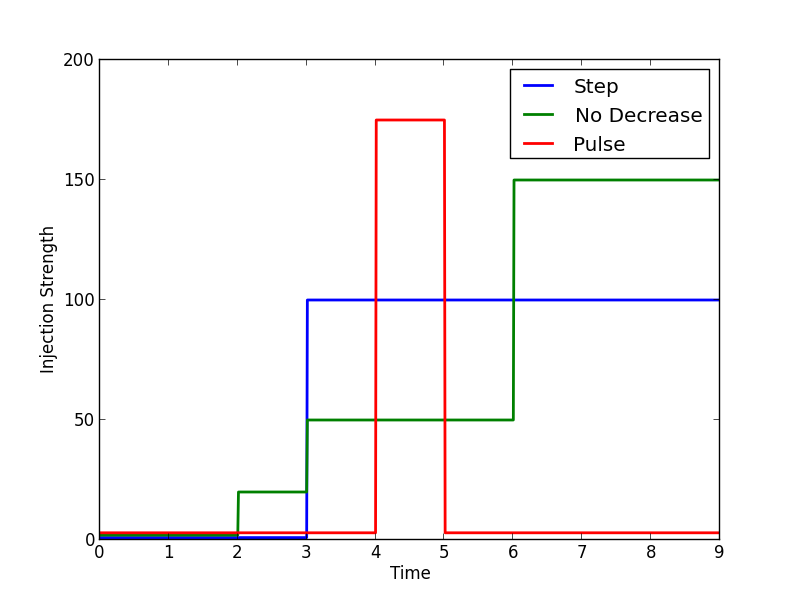
\includegraphics[scale=0.5]{graphics/inversion_injection_variation.png}
  \caption{Three different types of contamination injection profiles.}
  \label{fig:inversion_variations}

\end{figure}
             
The first variation of this formulation 
requires the injection to be a single step of any
calculated strength $S$ and can be run using the formulation option of
MIP\_discrete\_step in the inversion block. The Step profile shown in
Figure \ref{fig:inversion_variations} illustrates an example of this
type of injection. This variant is implemented by adding the following constraints to
the base formulation:

\begin{align}
&m_{n,t} \le S &&\forall n \in \mathbf{N}, t\in \mathbf{T} \\
&m_{n,t} \ge S - B(1-y_n) &&\forall n \in \mathbf{N}, t\in \mathbf{T}
\end{align}

The second variation adds constraint Equation \ref{eqn.mass_inj_constraint} 
to the base formulation to allow for
the case where the mass flow rate of the contaminant can stay the same
or increase with time. The No Decrease profile shown in
Figure \ref{fig:inversion_variations} gives an example of this kind of
injection. This variant of the formulation can be run using the
formulation option of MIP\_discrete\_nd in the inversion block.

\begin{align}
 &m_{n,t-1} \le m_{n,t} &&\forall n \in \mathbf{N}, t\in \mathbf{T}:
 j \neq 0 \label{eqn.mass_inj_constraint}
\end{align}

The third variation solves the Step formulation by fixing the binary
variable $y_n$ corresponding to a source node and solving the
resulting linear program (LP) for all nodes $n \in, N$. The objective
values for all LP solutions are compared and only a fraction of the
identified nodes are reported in the results based on
the candidate threshold option in inversion block of the configuration file. 
This LP variant can be run using the formulation option of
LP\_discrete in the inversion block.

\subsection{Bayesian Probability Based Formulation}
\label{sec.bayesian_algorithm}
This formulation calculates the probability of a node being the true
injection node using Bayes rule:
\begin{align}
P(i|m) = \frac{P(m|i)P(i)}{P(m)} \label{source_probability}
\end{align}
where contamination incident $i$ is an injection at a node and at a particular time step and $P(i|m)$ is 
the probability of an incident $i$ given a set of measurements $m$. Here, $P(i)$ is the 
prior probability of an incident. This formulation assumes that only a single injection 
incident is possible, and therefore it uses an uniform prior of 1/(all possible incidents). 
Since it is difficult to estimate $P(m)$ (the prior probability of a measurement), 
this calculation is substituted by obtaining the $P(i|m)$ for all possible incidents and 
then normalizing them to 1. Finally, $P(m|i)$ is the probability of a measurement 
given an injection incident. It is calculated using the following equation:


\begin{align}
P(m|i) = (1-p_f)^{\mathrm{match}(i)}p_f^{\mathrm{meas} - \mathrm{match}(i)}
\end{align}
where, $p_f$ is the probability of measurement failure, $\mathrm{meas}$ is the total number 
of measurements and $\mathrm{match}(i)$ is the number of discrete measurements that match the discrete concentrations 
obtained by simulating incident $i$. Note that calculating the discrete concentration profile 
obtained by simulating an incident requires a threshold that is specified by using the negative threshold option of the inversion block of the 
\code{inversion} configuration file.

After calculating the normalized probability $P(i|m)$ for all
incidents, only those having a probability above a confidence limit
are reported as the set of likely incidents along with their
corresponding $P(i|m)$ values. This
confidence limit is by default set to 95\% (0.95) and can be changed
by using the confidence option of the inversion block.

\subsection{Contaminant Status Algorithm (CSA)}
\label{sec.csa_algorithm}

The Contaminant Status Algorithm (CSA), proposed by \citet{csa},
performs source identification by assigning a status to each candidate
node-time pair as either being safe (not an injection candidate),
unsafe (possible injection candidate) or unknown. In WST, the CSA has
been modified to assign a likeliness measure of 1 to a node if it is
contained in the list of unsafe node-time pairs, while all other nodes
are assigned a likeliness measure of 0.

CSA uses a linear input-output water quality model generated through
the Particle Backtracking Approach (PBA) proposed
by \citet{Shang2002}. For every sensor $j$ and analysis time $t$, this
model provides the upstream reachability set, $U_j(t)$, that contains
the list of node-time pairs that are hydraulically connected to that
measurement. Using this set, a station source matrix, $S_j$, which
represents the list of safe, unsafe and unknown nodes based on all the
measurements available from sensor node $j$ only, is updated
iteratively using the following algorithm:

\begin{enumerate}
\item Initialize $S_j(i,\hat{t}) = $ Unknown, $\forall i \in \mathbf{N}, \forall \hat{t} \in \mathbf{T} $
\item For $(i,\hat{t}) \in U_j(t)$
        \begin{enumerate}
                \item For significant hydraulic connections (based on a threshold in the PBA input-output model)-
                        if the current measurement at sensor $j$ is positive, Set $S_j(i,\hat{t}) = $ Unsafe,
                        else Set $S_j(i,\hat{t}) = $ Safe
                \item For weak hydraulic connections (based on a threshold in the PBA input-output model), Set $S_j(i,\hat{t}) = $ Unknown
        \end{enumerate}
\end{enumerate}
where $N$ is the set of all candidate nodes and $T$ is the set of all
time steps in the time horizon. Based on the status from every
station source matrix, $S_j$, a total source status matrix $S$ that
contains the overall status of all candidate node-time pairs,
$(i,\hat{t})$, is updated using the following rules - an unsafe
node-time pair can only change to safe based on its corresponding
state in $S_j$; an unknown node-time pair can change to both safe or
unsafe; and if a node-time pair is safe, it will remain safe. Hence,
the total source status matrix is also updated iteratively over the
complete list of measurement time steps to obtain the final status of
all candidate injection node-time pairs. Consequently, CSA allows for
multiple simultaneous injections, however, it assumes perfect
measurements when marking candidate injections as safe.


\section{Source Identification Solvers}

The MIP algorithm builds an optimization formulation, and requires a MIP 
solver to perform source inversion. Therefore, if the MIP algorithm is selected 
(\code{algorithm:\ optimization}) as described in Section 
\ref{sec.inversion_subcommand.config_options}), then a solver needs to be 
specified. The solvers recognized by the \code{inversion} subcommand are 
the same as those recognized by \code{booster\_mip} subcommand (See 
Section \ref{booster_mip_solver} for more details).

\section{\code{inversion} Subcommand}\label{sec.inversion_subcommand}

The \code{inversion} subcommand is executed using the following
command line:
\begin{unknownListing}
wst inversion <configfile>
\end{unknownListing}
where \code{configfile} is a WST configuration file in the YAML format.

The \code{---help} option prints information about this subcommand,
such as usage, arguments and a brief description:
\begin{unknownListing}
wst inversion --help
\end{unknownListing}

\subsection{Configuration File}

The \code{inversion} subcommand generates a template configuration
file using the following command line:

\begin{unknownListing}
wst inversion --template <configfile>
\end{unknownListing}

The \code{inversion} template configuration file is shown in
Figure \ref{fig:inversion_template}. Brief descriptions of the
options are included in the template after the \# sign.

\begin{figure}[!ht]
  \unknownInputListing{examples/inversion_config.yml}{}{1}{35}
  \caption{The \code{inversion} configuration template file.}
  \label{fig:inversion_template}
\end{figure}

\subsection{Configuration Options}\label{sec.inversion_subcommand.config_options}

Full descriptions of the WST configuration options used by the \code{inversion} subcommand are listed below.
\begin{description}[topsep=0pt,parsep=0.5em,itemsep=-0.4em]
  \item[{network}]\hfill
  \begin{description}[topsep=0pt,parsep=0.5em,itemsep=-0.4em]
    \item[{epanet file}]\hfill
\\ The name of the EPANET 2.00.12 input (INP) file that defines the water distribution
                network model.
                
                Required input.
  \end{description}
  \item[{measurements}]\hfill
  \begin{description}[topsep=0pt,parsep=0.5em,itemsep=-0.4em]
    \item[{grab samples}]\hfill
\\The name of the file that contains all the measurements from 
                the manual grab samples and the fixed sensors. The measurement file 
                format is documented in File Formats Section \ref{formats_measFile}.

                Required input.
  \end{description}
  \item[{inversion}]\hfill
  \begin{description}[topsep=0pt,parsep=0.5em,itemsep=-0.4em]
    \item[{algorithm}]\hfill
\\The algorithm used to perform source inversion. The options are 
				optimization, bayesian, or csa. The optimization algorithm requires 
				AMPL or PYOMO along with a MIP solver. The bayesian algorithm 
				uses Bayes' Rule to update probability of a particular node 
				being the contaminant source node. The CSA is the Contaminant
                                Status Algorithm by \citet{csa}.
                
                Required input, default = optimization.
    \item[{formulation}]\hfill
\\The formulation used by the optimization algorithm. The options are 
                LP\_discrete (discrete LP), MIP\_discrete (discrete MIP), 
                MIP\_discrete\_nd (discrete MIP with no decrease) or 
                MIP\_discrete\_step (discrete MIP for step injection).
                
                Required input for optimization algorithm, default = MIP\_discrete.
    \item[{model format}]\hfill
\\The modeling language used to build the formulation specified
                by the formulation option. The options are AMPL and PYOMO. 
				AMPL is a third party package that must be installed by 
				the user if this option is specified. PYOMO is an open source 
				software package that is distributed with WST.
                
                Required input for optimization algorithm, default = PYOMO.
    \item[{merlion water quality model}]\hfill
\\This option is set to true to use the Merlion 
                water quality model for simulating the candidate injections
                in the Bayesian probability-based method. It can be set to false
                to use EPANET 2.00.12 for these simulations. Note that the Merlion water quality
                model is required in either case to generate the initial list of candidate injections.
 
                Optional input, default = true.
    \item[{horizon}]\hfill
\\The minutes over which the past measurement
                data is used for source inversion. It is calculated backwards from
                the latest measurement time in the measurements file. 
                All measurements in the measurements file that are within the horizon 
                are used (both negative and positive). In the case of the CSA algorithm, 
                the implementation assumes fixed sensors only, and all measurements at 
                these sensors are assumed to be negative prior to the horizon.
                If the horizon is longer
                than the time between the latest measurement and simulation start time,
                then all the measurements are used for source inversion.
                
                Required input, default = None (Start of simulation).
    \item[{num injections}]\hfill
\\The number of possible injections to consider when
                performing inversion. Multiple injections are only supported by
                the MIP formulation. This value must be set to 1 for the LP model
                or the probability algorithm.
                
                Required input for optimization algorithm, default = 1.
    \item[{measurement failure}]\hfill
\\The probability that a sensors gives an incorrect reading. Must be between 0 and 1. 
                
                Required input for the Bayesian algorithm, default = 0.05.
    \item[{positive threshold}]\hfill
\\The concentration threshold used by the sensors to flag a positive 
                detection measurement. This is a parameter in the optimization algorithm (Equation \ref{eqn.milp_positive_set}).
                
                Required input for optimization algorithm, default = 100 mg/L. 
    \item[{negative threshold}]\hfill
\\The concentration threshold used by the sensors to flag
                a negative detection measurement. This is a parameter in the
                optimization algorithm (Equation \ref{eqn.milp_negative_set}).
                
                Required input for optimization algorithm, default = 0.0 mg/L.
    \item[{feasible nodes}]\hfill
\\A list that defines nodes that can be considered for the source inversion problem.
                The options are: (1) ALL, which specifies all nodes as feasible source locations;
                (2) NZD, which specifies all non-zero demand nodes as feasible source locations;
                (3) a list of EPANET node IDs, which identifies specific nodes as feasible source locations; or
                (4) a filename, which is a space or comma separated file containing a list of 
                specific nodes as feasible source locations. 

                Optional input.
    \item[{candidate threshold}]\hfill
\\The objective cut-off value for candidate contamination incidents 
                using the optimization algorithm. The objective value represents the
                likelihood of a particular node being the injection node (See Equation \ref{eq_transform_obj}).  
                The objective values are normalized to 1 and only the nodes having 
                their objective values greater or equal to the threshold are reported
                in the inversion results. 
                
                Required input for optimization algorithm, default = 0.20.
    \item[{confidence}]\hfill
\\The probability cut-off value for candidate contamination incidents
                using the Bayesian algorithm. The value is between 0 and 1. 
                
                Required for the Bayesian algorithm, default = 0.95.
    \item[{output impact nodes}]\hfill
\\A option to output a Likely\_Nodes.dat file that contains only
                the node IDs of the possible contaminant injection nodes obtained from the 
                \code{inversion} subcommand. This file can be used as the feasible nodes for the next 
                iteration of the \code{inversion} subcommand to only consider this set of possible contaminant 
                injection nodes.
                
                Optional input, default = false.
  \end{description}
  \item[{solver}]\hfill
  \begin{description}[topsep=0pt,parsep=0.5em,itemsep=-0.4em]
    \item[{type}]\hfill
\\The solver type. Each component of WST
				(e.g., sensor placement, flushing response, booster 
				placement) has different 
				solvers available. More specific details are provided in 
				the subcommand's chapter.
                
                Required input.
    \item[{options}]\hfill
\\A list of options associated with a specific solver type. More
            information on the options available for a specific solver
            is provided in the solver's documentation. The Getting
            Started Section \ref{dependencies} provides links to the
            different solvers.
            
            Optional input.
    \item[{threads}]\hfill
\\The maximum number of threads or function evaluations the solver is
                allowed to use.  This option is not available to all solvers or all analyses.
                
                Optional input.
    \item[{logfile}]\hfill
\\The name of a file to output the results of the solver.
                
                Optional input.
    \item[{verbose}]\hfill
\\The solver verbosity level.
                
                Optional input, default = 0 (lowest level).
    \item[{initial points}]\hfill
    \begin{description}[topsep=0pt,parsep=0.5em,itemsep=-0.4em]
      \item[{nodes}]\hfill
\\A list of node locations (EPANET IDs) to begin the optimization
        process. Currently, this option is only supported for the
        network solver used in the flushing and booster\_msx
        subcommands. This input causes an error for other subcommands.
        
        Optional input.
      \item[{pipes}]\hfill
\\A list of pipe locations (EPANET IDs) to begin the optimization
        process. Currently, this option is only supported for the
        network solver used in the flushing subcommand. This input causes an error for other subcommands.
        
        Optional input.
    \end{description}
  \end{description}
  \item[{configure}]\hfill
  \begin{description}[topsep=0pt,parsep=0.5em,itemsep=-0.4em]
    \item[{output prefix}]\hfill
\\The prefix used for all output files.
                
                Required input.
    \item[{output directory}]\hfill
      \\The output directory to store the results.
    \item[{debug}]\hfill
\\The debugging level (0 or 1) that indicates the amount of debugging 
                information printed to the screen, log file and output yml file. 
                
                Optional input, default = 0 (lowest level).
  \end{description}
\end{description}


\subsection{Subcommand Output}
% The <output prefix>inversion.json file contains a summary of 
% the \code{inversion} subcommand results. This file includes a list of
% node locations along with their objective or probability values, in 
% which a higher value indicates a higher likelihood of that node being 
% the true contaminant injection node.  The injection profiles (start 
% and end times and the strength) for each possible injection node are 
% also included along with the run date and CPU time for inversion.
% The \code{inversion} subcommand also outputs an 
% <output prefix>profiles.tsg file that contains the list of likely 
% injection profiles in the TSG file format (See File Formats 
% Section \ref{formats_tsgFile}). As discussed in Chapter \ref{chap:grabsample}, this TSG
% file can be directly used as an input by the \code{grabsample} 
% subcommand.

The \code{inversion} subcommand creates several output files. 
The YAML file called <output prefix>inversion\_output.yml 
contains a list of possible source node locations (EPANET node IDs),  
the associated objective or probability value (node likeliness) for each possible source node 
(a higher value indicates a higher likelihood of that node being 
the true contaminant injection node), the injection profiles (start 
and end times and the strength) for each possible source node, 
the run date and CPU time. 
The log file called <output prefix>inversion\_output.log contains basic debugging information. 
The \code{inversion} subcommand also outputs an 
<output prefix>\_profile.tsg file that contains the list of likely 
injection profiles in the TSG file format (See File Formats 
Section \ref{formats_tsgFile}). As discussed in Chapter \ref{chap:grabsample}, this TSG
file can be directly used as an input by the \code{grabsample} 
subcommand.
A visualization YAML configuration file named <output prefix>inversion\_output\_vis.yml is also created.
The \code{visualization} subcommand is automatically run using this YAML file.

\section{Source Identification Examples}
Three examples illustrating the use of the different source identification
methods available in WST are presented. In the first example, the optimization
formulation is used to solve a source identification problem, while the
second example uses the Bayesian probability formulation and the third example 
uses the Contaminant Status Algorithm (CSA) to solve the exact same problem. 
An EPANET 2.00.12 network model (INP format) and a measurements file (See File
Formats Section \ref{formats_measFile}) are required to run
the \code{inversion} subcommand. 

Since real system data is not available, a measurements file required for
the \code{inversion} subcommand can be generated using
the \code{measuregen} executable (Executable Files Section \ref{measuregenExecutable}). 
The three examples use the EPANET Example Network 3 input file (Net3.inp) 
as the network file, which runs a two day hydraulic and water
quality simulation. An injection at node 151 is simulated 
from 8 hours until 24 hours, specified using
the Net3\_inversion.tsg file. The sensor locations are provided using
the Net3\_fixed\_sensors file, and the measurements are obtained every
15 minutes with a concentration threshold of 0 indicating
contamination. The following command line statement can be run from
the examples folder to generate the measurements file:

\begin{unknownListing}
measuregen --inp=Net3/Net3.inp --tsg=Net3/Net3_inversion.tsg --start-sensing-time=0 
--stop-sensing-time=705 --measures-per-hour=4 --threshold=0 --ignore-merlion-warnings 
--output-prefix=Net3/Net3 Net3/Net3_fixed_sensors
\end{unknownListing}

The resulting Net3\_MEASURES.dat file is used in the following three examples. 

\subsection{Example 1}  
In the first example, the optimization method is used to solve 
the source identification problem. The configuration file, 
inversion\_ex1.yml, shown in Figure \ref{fig:inversion_ex1} is used to
identify the possible contaminant source locations. The MIP
optimization formulation, MIP\_discrete\_step, is used for this
example. The example uses the Net3\_MEASURES.dat file
generated using the \code{measuregen} executable.

\begin{figure}[!ht]
  \unknownInputListing{../../examples/inversion_ex1.yml}{}{1}{26}
  \caption{The \code{inversion} configuration file for example 1.}
  \label{fig:inversion_ex1}
\end{figure}

The example can be executed using the following command line:
\begin{unknownListing}
wst inversion inversion_ex1.yml
\end{unknownListing}

The results are contained in the file {\outputprefix}inversion\_output.yml.
A section of this results file is shown in
Figure \ref{fig:inversion_ex1_re}. The results contain a list of sets
where each set contains - possible contaminant source node in the
Nodes list (which contains a node Name and a Profile), CPU
computation time in seconds and the Objective value corresponding
to the solution which identifies that node as the source node. The
Objective value for each candidate node $n$ in the results file is
related to the objective of the MIP
formulations \ref{sec.mip_formulation}
(Equation \ref{eqn.milp_first_egn}). The objective calculated from the
MIP formulation is transformed such that it is normalized to 1 and a
higher value means a higher likelihood of a node being the source
node. This transformation is done by the following equations:
\begin{align}
\textrm{INV\_NORM\_OBJ}_n &= 1 - \frac{\textrm{FORM\_OBJ}_n}{\max(\textrm{FORM\_OBJ})} &&\forall n \in \mathbf{N}\\
\textrm{Objective}_n &= \frac{\textrm{INV\_NORM\_OBJ}_n}{\max(\textrm{INV\_NORM\_OBJ})} &&\forall n \in \mathbf{N} \label{eq_transform_obj}
\end{align}
where $\textrm{FORM\_OBJ}_n$ (Formulation Objective) is the objective
value as calculated from the MIP formulation
Equation \ref{eqn.milp_first_egn} when node $n$ is identified as the
most likely node, $\textrm{INV\_NORM\_OBJ}_n$ is an intermediate
variable that represents one (1) minus the normalized formulation objective
and $\textrm{Objective}_n$ is the normalized form of the
$\textrm{INV\_NORM\_OBJ}_n$ which is reported in the \code{inversion}
subcommand results file.
   
This results file only contains the list
of possible contaminant source nodes that have an objective (as calculated by \ref{eq_transform_obj}) greater
than the candidate threshold provided in the inversion block of the WST configuration
file. 

\begin{figure}[!ht]
  \unknownInputListing{examples/inversion/inversion_ex1_output.yml}{}{1}{15}
  \caption{The \code{inversion} YAML output file for example 1.}
  \label{fig:inversion_ex1_re}
\end{figure}

For this example scenario, the \code{inversion} subcommand is able to
correctly identify node 151 as one of the three most likely source
nodes. This means that given the current measurement information
available, nodes 151, 153 and 149 are equally likely. Further
measurements can be obtained from selected grab sampling locations that
can help in distinguishing between these three potential source
nodes. 
An example of how to use the \code{grabsample} subcommand to
optimally select grab sampling location to improve the identification of the 
true contamination source is provided in the source identification case study 
in the Advanced Topics and Case Studies chapter \ref{inversion_case_study}.

\subsection{Example 2}  
In this example, the Bayesian probability formulation is used to solve
the same problem described in example 1. The configuration file,
inversion\_ex2.yml, shown in Figure \ref{fig:inversion_ex2}, is used for
this example. The bayesian formulation is selected
by using the algorithm option in the inversion
block.
 
\begin{figure}[!ht]
  \unknownInputListing{../../examples/inversion_ex2.yml}{}{1}{26}
  \caption{The \code{inversion} configuration file for example 2.}
  \label{fig:inversion_ex2}
\end{figure}


The example can be executed using the following command line:
\begin{unknownListing}
wst inversion inversion_ex2.yml
\end{unknownListing}

The results are contained in the file {\outputprefix}inversion\_output.yml
shown in Figure \ref{fig:inversion_ex2_re}. The likeliness value
reported in this file corresponds to the probability value calculated
by Equation \ref{source_probability}. The probability algorithm is
also able to correctly identify node 151 as the one of the three most
probable source nodes along with nodes 149 and 153. 

\begin{figure}[!ht]
  \unknownInputListing{examples/inversion/inversion_ex2_output.yml}{}{1}{13}
  \caption{The \code{inversion} YAML output file for example 2.}
  \label{fig:inversion_ex2_re}
\end{figure}

\subsection{Example 3}  
In this example, the Contaminant Status Algorithm (CSA) is used to solve
the same problem described in example 1. The configuration file,
inversion\_ex3.yml, shown in Figure \ref{fig:inversion_ex3}, is used for
this example. CSA is selected
by using the algorithm option in the inversion
block.
 
\begin{figure}[!ht]
  \unknownInputListing{../../examples/inversion_ex3.yml}{}{1}{26}
  \caption{The \code{inversion} configuration file for example 3.}
  \label{fig:inversion_ex3}
\end{figure}


The example can be executed using the following command line:
\begin{unknownListing}
wst inversion inversion_ex3.yml
\end{unknownListing}

The results are contained in the file
{\outputprefix}inversion\_output.yml shown in
Figure \ref{fig:inversion_ex3_re}. Since in WST, a
likeliness measure of 1 is assigned to a node if it is contained in the list of
unsafe node-time pairs, while a likeliness measure of 0 is assigned to all other nodes, 
the node likeliness in the results output file is 1.0 for all possible contamination injection nodes. 
CSA is also able to correctly identify node 151 as the one of the four most probable
source nodes along with nodes 125, 149 and 153.

\begin{figure}[!ht]
  \unknownInputListing{examples/inversion/inversion_ex3_output.yml}{}{1}{13}
  \caption{The \code{inversion} YAML output file for example 3.}
  \label{fig:inversion_ex3_re}
\end{figure}


